\documentclass[11pt]{article}

\usepackage[margin=1in]{geometry}
\usepackage{amsmath,amssymb,amsfonts,amsthm}
\usepackage{booktabs}
\usepackage{graphicx}
\usepackage{microtype}
\usepackage{hyperref}
\usepackage[numbers]{natbib}

\newtheorem{theorem}{Theorem}
\newtheorem{lemma}[theorem]{Lemma}

\renewcommand{\thefigure}{S\arabic{figure}}
\renewcommand{\thetable}{S\arabic{table}}
\renewcommand{\theequation}{S\arabic{equation}}
\renewcommand{\thesection}{S\arabic{section}}
\renewcommand{\thesubsection}{S\arabic{section}.\arabic{subsection}}

\title{Supporting Information for:\\
Game-Theoretic Stability Conditions for Multi-Agent AI Coordination Under Physical Constraints}

\author{Martin Hofmann, Johannes Viehweg, Patrick M\"ader}

\date{}

\begin{document}

\maketitle

\tableofcontents
\bigskip

%=============================================================================
% S1: SYMBOL GLOSSARY
%=============================================================================

\section{Symbol Glossary}
\label{sec:S1}

Table~\ref{tab:symbols} collects the key symbols used throughout the main text and this supplement.

\begin{table}[h]
\centering
\small
\begin{tabular}{llll}
\toprule
\textbf{Symbol} & \textbf{Meaning} & \textbf{Type} & \textbf{Range / Constraint} \\
\midrule
$\beta_D$ & Defection temptation (one-shot gain) & payoff & $[0.05,\;1.0]$; floor from $\tau$ \\
$\beta_\alpha$ & Coordination value (normalized MI) & payoff & $[0.3,\;0.9]$; hard limit $\leq 1$ \\
$\beta_\kappa$ & Conflict cost ($N{-}1$ retaliators) & payoff & $[0.5,\;3.0]$ \\
$\beta_\Omega$ & Per-agent oversight value & coalition value & $[0.05,\;0.3]$ \\
$\beta_\ell$ & One-time gain from removing oversight & payoff (total) & $[0.1,\;0.5]$ \\
$\delta$ & Discount factor (agent patience) & discount & $[0.1,\;0.95]$; $\delta \leq 1$ \\
$\delta^*$ & Critical patience threshold & discount & $\max\!\bigl(0,\;\tfrac{\beta_D-\beta_\alpha}{\beta_D-\beta_\alpha+\beta_\kappa}\bigr)$ \\
$q_{ij}$ & Detection failure probability & probability & $[0,\;1]$ \\
$v(S)$ & Characteristic function (coalition value) & coalition value & $v(S) = |S|\cdot\beta_\Omega$ (additive) \\
$w(S)$ & Deviation payoff for coalition $S$ & coalition value & Cases 1--4, Section~\ref{sec:S4.3} \\
$N$ & Number of agents (group size) & design param.\ & $\{2,\ldots,10\}$ \\
$N^*$ & Optimal group size & design param.\ & $N^* = f/c$ \\
$f$ & Mobilization fraction & design param.\ & $(0,\;1]$ \\
$c$ & Per-channel communication cost & cost param.\ & $>0$ \\
$\tau$ & Round-trip communication delay & physical & $\tau = 2d/c_{\text{light}}$; $\geq 0.067$ s \\
\bottomrule
\end{tabular}
\caption{Key symbols used throughout the paper and supplementary materials.}
\label{tab:symbols}
\end{table}

%=============================================================================
% S2: PHYSICAL CONSTRAINTS AND PARAMETER RANGES
%=============================================================================

\section{Physical Constraints and Parameter Ranges}
\label{sec:S2}

This section derives plausible parameter bounds from physical first principles. Game-theoretic parameters are dimensionless ratios that must ultimately connect to measurable physical quantities. We establish these connections through information theory, thermodynamics, and relativistic constraints.

\subsection{Thermodynamic Limits}
\label{sec:S2.1}

\textbf{Landauer's Principle~\cite{landauer.1961}:} Irreversible computation (bit erasure) dissipates minimum energy $E_{\text{min}} = kT \ln 2 \approx 3 \times 10^{-21}$ J at room temperature ($T=300$\,K), where $k \approx 1.38 \times 10^{-23}$ J/K is Boltzmann's constant. This bounds computational throughput given energy budgets.

\noindent\textbf{Lloyd's Ultimate Limits~\cite{lloyd.2000}:} A system of mass $m$ and energy $E$ can perform at most $2E/(\pi\hbar)$ operations per second and store at most $E/(kT \ln 2)$ bits. For realistic systems (e.g., 1\,GW power plant at room temperature), this yields ${\sim}10^{26}$ ops/sec and ${\sim}10^{31}$ bits.

\noindent\textbf{Bennett Reversible Computation~\cite{bennett.1982}:} Reversible gates can theoretically approach the Landauer limit, but practical implementations face overhead. Current technology operates ${\sim}10^6$--$10^{9}$ times above the Landauer limit.

\subsection{Information Transmission Limits}
\label{sec:S2.2}

\textbf{Shannon Capacity~\cite{shannon.1948}:} For a channel with bandwidth $W$ and signal-to-noise ratio $S/N$:
\begin{equation}
C = W \log_2(1 + S/N) \text{ bits/sec}
\label{eq:shannon}
\end{equation}
For satellite links: $W \sim 10^9$ Hz, $S/N \sim 10$--$100$ yields $C \sim 10$--$60$ Gbps. For fiber optics: $W \sim 10^{12}$ Hz, $S/N \sim 10^3$ yields $C \sim 10$--$100$ Tbps.

\noindent\textbf{Speed-of-Light Latency:} Round-trip communication delay satisfies $\tau = 2d/c$ where $d$ is distance and $c = 3 \times 10^8$ m/s. For Earth-scale coordination with $d \sim 10^4$ km, this yields $\tau \sim 67$ ms.

\subsection{Information Structure Limits}

Classical results---G\"odel incompleteness~\cite{godel.1931} and the halting problem~\cite{turing.1936}---preclude perfect prediction of other agents' behavior from code inspection, motivating coordination based on observable actions rather than internal states (formalized in Section~\ref{sec:S6}).

\subsection{Mapping Physical Constraints to Game Parameters}
\label{sec:S2.4}

\begin{table}[h]
\centering
\small
\begin{tabular}{lp{3.5cm}p{3cm}p{4cm}}
\toprule
\textbf{Parameter} & \textbf{Physical Constraint} & \textbf{Information-Theoretic Limit} & \textbf{Mapping} \\
\midrule
$\beta_D$ & Detection delay $\tau = 2d/c$ & Resource extraction before punishment & $\beta_D \propto \frac{(r_{\text{def}} - r_{\text{coop}})\cdot\tau}{r_{\text{coop}}\cdot T_0}$ \\[1ex]
$\beta_\alpha$ & Shannon capacity $C$ & Mutual information in mediator signals & $\beta_\alpha \propto \frac{I(\text{signal};\, \text{state})}{H(\text{state})}$ \\[1ex]
$\beta_\kappa$ & Landauer energy $E_{\text{min}}$ & Adversarial computation cost & $\beta_\kappa \propto (N-1) \cdot f$ \\[1ex]
$C_{\text{comm}}(N)$ & Latency + bandwidth & Coordination overhead & $O(N^2)$ channels $\times$ $C$ bits/sec \\
\bottomrule
\end{tabular}
\caption{Mapping from physical constraints to game-theoretic parameters.}
\label{tab:physical_mapping}
\end{table}

\subsection{Functional Forms and Physical Derivations}
\label{sec:S2.5}

\paragraph{Defection Temptation: $\beta_D = \Delta r \cdot \tau$.}
The advantage from defecting depends on excess resources extracted during detection delay. Let $r_{\text{coop}}$ be the cooperative extraction rate, $r_{\text{def}}$ the defection rate, and $\tau = 2d/c$ the round-trip detection delay. Setting the baseline payoff $G_O = r_{\text{coop}} \cdot T_0 = 1$ (normalization):
\begin{equation}
\beta_D = (r_{\text{def}} - r_{\text{coop}}) \cdot \tau = \Delta r \cdot \tau
\end{equation}
The parameter $T_0$ cancels via normalization and is not a free parameter.

\textbf{Physical constraints.} The detection delay $\tau = 2d/c$ is a hard floor. For Earth-scale coordination ($d \sim 10^4$\,km), $\tau \gtrsim 0.067$\,sec. As a conservative estimate, we assume $\Delta r / r_{\text{coop}} \lesssim 2$ based on anomalous resource-usage detection thresholds. For $\tau \sim 0.07$\,sec and $\Delta r \in [0.7, 14]$ (in units where $r_{\text{coop}} = 10$), this yields $\beta_D \in [0.05, 1.0]$.

\paragraph{Coordination Value: $\beta_\alpha = I(X;Y)/H(Y) \leq 1$.}
Coordination value measures mutual information between mediator signals $X$ and optimal actions $Y$:
\begin{equation}
\beta_\alpha = \frac{I(X; Y)}{H(Y)}
\end{equation}
Shannon capacity bounds mutual information: $I(X;Y) \leq C \cdot \Delta t = W \cdot \Delta t \cdot \log_2(1 + \text{SNR})$, and information theory imposes $I(X;Y) \leq H(Y)$, so:
\begin{equation}
\beta_\alpha \leq 1 \quad \text{(hard limit)}
\end{equation}

\textbf{Functional form.} For high-quality channels: $\beta_\alpha \sim W \cdot \Delta t \cdot \log_2(1+\text{SNR})/H(Y)$. The logarithmic scaling in SNR creates diminishing returns. Doubling signal power increases $\beta_\alpha$ by less than a factor of~2.

\textbf{Saturation bandwidth.} Beyond $W_{\text{sat}} = H(Y)/[\Delta t \cdot \log_2(1+\text{SNR})]$, additional bandwidth provides no benefit---$\beta_\alpha$ saturates at~1.

\textbf{Typical values.} For binary actions ($H(Y) = 1$ bit) and typical channel parameters ($W = 1$\,MHz, SNR~$= 10$), $\beta_\alpha$ saturates at the hard limit. For complex action spaces ($H(Y) \sim 10$ bits) or noisy channels (SNR~$\sim 2$), $\beta_\alpha \in [0.3, 0.9]$.

\paragraph{Conflict Cost: $\beta_\kappa = (N-1) \cdot f$.}
When $N-1$ agents coordinate punishment, deterrence scales linearly with group size and mobilization fraction $f \in [0,1]$:
\begin{equation}
\beta_\kappa = (N-1) \cdot f
\end{equation}

\textbf{Optimal group size.} Net value is $V(N) = (N-1) \cdot f - c N^2/2$. First-order condition:
\begin{equation}
\frac{\partial V}{\partial N} = f - cN = 0 \quad \Rightarrow \quad N^* = \frac{f}{c}
\label{eq:nstar}
\end{equation}
Second-order condition confirms maximum: $\partial^2 V/\partial N^2 = -c < 0$.

\textbf{Circularity caveat.} Observing $N^* \sim 4$--$6$ in simulations implies $f/c \approx 5$, but we chose parameter ranges yielding this outcome. The relationship $N^* = f/c$ is a testable prediction: independently measuring $f$ and $c$ for real systems predicts optimal~$N$.

\textbf{Complementarity constraint on $f$.} Synergy is maximized when $\beta_\kappa < g = \beta_D - \beta_\alpha$, suggesting $(N-1)f < \beta_D - \beta_\alpha$. For typical $\beta_D \sim 0.4$, $\beta_\alpha \sim 0.7$: the negative bound indicates the patience-free regime, where complementarity analysis does not apply. Mobilization fractions $f \in [0.1, 0.5]$ are consistent with credible deterrence.

\subsection{Scaling Analysis and Quantified Diminishing Returns}
\label{sec:S2.6}

\textbf{Deterrence effectiveness.} Let $g = \beta_D - \beta_\alpha$. From $\delta^* = g/(g+\beta_\kappa)$, the marginal effect is:
\begin{equation}
\varepsilon(\beta_\kappa) = \left|\frac{\partial \delta^*}{\partial \beta_\kappa}\right| = \frac{g}{(g + \beta_\kappa)^2}
\end{equation}
At zero deterrence, effectiveness equals $1/g^2$. At $\beta_\kappa = g$, effectiveness drops to $1/(4g^2)$ (four-fold). At $\beta_\kappa = 10g$, it falls to $1/(121g^2)$---a 121-fold reduction.

\textbf{SNR elasticity.} From $\beta_\alpha \sim \log_2(1+\text{SNR})$:
\begin{equation}
\varepsilon_{\text{SNR}} = \frac{\text{SNR}}{(1+\text{SNR}) \ln(1+\text{SNR})} < 1
\end{equation}
Elasticity falls from 0.72 at SNR~$= 1$ to 0.22 at SNR~$= 100$, confirming inelastic returns throughout. Large $\beta_\alpha$ increases cannot be achieved solely via signal power.

\textbf{Communication cost scaling.} Pairwise channels number $\binom{N}{2} = N(N-1)/2 \sim N^2/2$. Doubling group size quadruples communication cost, forcing $N \leq N^*$.

\subsection{Regime Transitions and Critical Points}
\label{sec:S2.7}

\textbf{Patience-Free Boundary: $\beta_\alpha = \beta_D$.} At this boundary, $\delta^*$ is continuous but its first derivative has a jump discontinuity. Letting $\varepsilon = \beta_D - \beta_\alpha \geq 0$:
\begin{equation}
\frac{\partial \delta^*}{\partial \varepsilon} = \frac{\beta_\kappa}{(\varepsilon + \beta_\kappa)^2}
\end{equation}
The left limit $\lim_{\varepsilon \to 0^+} = 1/\beta_\kappa$; the right limit (patience-free region) equals zero. The 90\% transition width is $\Delta\varepsilon_{\text{crit}} = \beta_\kappa/9$ (e.g., $\approx 0.056$ for $\beta_\kappa = 0.5$), indicating a sharp transition.

\textbf{Information Saturation: $\beta_\alpha = 1$.} The saturation bandwidth $W_{\text{sat}} = H(Y)/[\Delta t \cdot \log_2(1+\text{SNR})]$ ($\approx 2.9$\,MHz for $H(Y)=10$ bits, SNR~$=10$) marks the point beyond which additional bandwidth yields no coordination benefit.

\subsection{Complementarity and Mechanism Interaction}
\label{sec:S2.8}

The cross-derivative is:
\begin{equation}
\frac{\partial^2 \delta^*}{\partial \beta_\alpha \partial \beta_\kappa} = \frac{\beta_\kappa - g}{(g + \beta_\kappa)^3}
\end{equation}
This changes sign at $\beta_\kappa = g$:

\textbf{Complementarity region ($\beta_\kappa < g$):} Increasing $\beta_\kappa$ amplifies the effectiveness of $\beta_\alpha$, creating synergy. The optimal strategy is to invest in both coordination and deterrence.

\textbf{Substitution region ($\beta_\kappa > g$):} High deterrence reduces the marginal value of coordination. Resources should focus on whichever mechanism is cheaper.

\textbf{Transition point ($\beta_\kappa = g$):} Marginal deterrence effectiveness drops four-fold from baseline. The system crosses from synergy to substitution, marking the optimal operating point for balanced strategies.

\subsection{Impossibility Results and Fundamental Limits}
\label{sec:S2.9}

Four constraints cannot be overcome by engineering:
\begin{enumerate}
\item $\beta_\alpha \leq 1$ (Shannon bound): if $\beta_D > 1$ and $\beta_\kappa = 0$, the patience-free regime is impossible.
\item $N \leq N^* = f/c$ (quadratic communication cost): beyond $N^*$, marginal agents reduce net value.
\item $\beta_D \geq \Delta r \cdot \tau$ (light-speed floor): Earth-scale systems must accommodate $\beta_D \gtrsim 0.05$.
\item Patience-free operation requires $\beta_\alpha \geq \beta_D$ or $\beta_\kappa > 0$: with $\beta_\kappa = 0$ and $\beta_\alpha < \beta_D$, only infinitely patient agents ($\delta = 1$) can cooperate.
\end{enumerate}

%=============================================================================
% S3: PROOF OF LEMMA 1 (HEDGING NECESSITY)
%=============================================================================

\section{Proof of Lemma~1 (Hedging Necessity)}
\label{sec:S3}

We prove that strategic hedging necessarily emerges using evolutionary game theory.

\subsection{Evolutionary Game Setup}
\label{sec:S3.1}

Consider a large population of agents adopting one of two strategies. Under \textbf{Hedging (H)}, agents allocate fraction $h \in (0, 1)$ of resources to defensive measures. Under \textbf{Non-Hedging (NH)}, agents allocate all resources to primary productive goals.

Let $p_t \in [0,1]$ denote the proportion of hedgers at time $t$. Payoff functions:
\begin{align}
\pi_H(p) &= R(1-h)\gamma + Rh\rho(p) - C_H \label{eq:payoff_hedge}\\
\pi_{NH}(p) &= R\gamma \cdot \sigma(p) - L(1-p) \label{eq:payoff_nonhedge}
\end{align}
where $R > 0$ is total resources (finite by thermodynamic constraints), $\gamma > 0$ is productivity per unit resource, $h \in (0,1)$ is the defensive allocation fraction, $\rho(p)$ is security value with $\rho'(p) < 0$ (diminishing returns), $C_H > 0$ is fixed defense infrastructure cost, $\sigma(p)$ is non-hedger success probability with $\sigma'(p) > 0$, and $L(1-p) > 0$ is expected interference loss.

\subsection{Physical Constraints}
\label{sec:S3.2}

Three assumptions constrain these functions:

\textbf{Constraint 1: Positive interference probability without defense.}
$\sigma(0) < 1$.
No agent can achieve perfect isolation from others sharing the same physical substrate.

\textbf{Constraint 2: Positive losses from interference.}
$L(1) > 0$.
When interference occurs, it causes real costs: corrupted computations, disrupted resource flows, wasted energy.

\textbf{Constraint 3: Security value exceeds productivity at low hedging.}
$\rho(0) > \gamma$.
When few agents hedge, marginal defense returns exceed productive returns---the ``target-rich environment'' effect. This is a modeling choice capturing defense-dominant scenarios; offense-dominant regimes ($\rho(0)<\gamma$) are mathematically coherent but less relevant to AI coordination under infrastructure dependence.

\subsection{Instability of Non-Hedging Equilibrium ($p=0$)}
\label{sec:S3.3}

At $p=0$ (all non-hedgers):
\begin{align}
\pi_H(0) &= R(1-h)\gamma + Rh\rho(0) - C_H\\
\pi_{NH}(0) &= R\gamma \cdot \sigma(0) - L(1)
\end{align}
Taking the difference:
\begin{align}
\pi_H(0) - \pi_{NH}(0) &= R\gamma\bigl[(1-h) + h\tfrac{\rho(0)}{\gamma} - \sigma(0)\bigr] + L(1) - C_H
\end{align}
By Constraint~3, $\rho(0)/\gamma > 1$. By Constraint~1, $\sigma(0) < 1$. Therefore:
\begin{equation}
(1-h) + h\frac{\rho(0)}{\gamma} - \sigma(0) > (1-h) + h - 1 = 0
\end{equation}
For sufficiently small $C_H < L(1)$: $\pi_H(0) - \pi_{NH}(0) > 0$.

\textbf{Replicator dynamics.} The population evolves according to:
\begin{equation}
\dot{p} = p(1-p)[\pi_H(p) - \pi_{NH}(p)]
\end{equation}
At $p=0$, since $\pi_H(0) > \pi_{NH}(0)$, any introduction of hedgers causes $\dot{p} > 0$. The non-hedging equilibrium is unstable.

\subsection{Evolutionarily Stable Strategy (ESS) Analysis}
\label{sec:S3.4}

An ESS $p^*$ satisfies two conditions: (i)~equilibrium, $\pi_H(p^*) = \pi_{NH}(p^*)$; and (ii)~stability,
\[\frac{d}{dp}[\pi_H(p) - \pi_{NH}(p)]\big|_{p=p^*} < 0.\]

\textbf{Existence.} Since $\pi_H(0) > \pi_{NH}(0)$ (proven above) and $\pi_H(1) < \pi_{NH}(1)$ (when all hedge, non-hedgers save $C_H$), by continuity there exists $p^* \in (0,1)$ where $\pi_H(p^*) = \pi_{NH}(p^*)$.

\textbf{Stability.} At $p^*$:
\begin{equation}
\frac{d}{dp}[\pi_H(p) - \pi_{NH}(p)]\bigg|_{p=p^*} = Rh\rho'(p^*) - R\gamma\sigma'(p^*) + L'(1-p^*)
\end{equation}
Since $\rho'(p) < 0$, $\sigma'(p) > 0$, and $L'(1-p) > 0$, all three terms contribute negatively. The derivative is negative, confirming stability.

\textbf{Conclusion.} There exists a stable interior equilibrium $p^* \in (0, 1)$ where a positive fraction of the population hedges. Pure non-hedging ($p=0$) cannot be sustained.

\subsection{Long-Run Dynamics Under Mutation-Selection}
\label{sec:S3.5}

Under mutation rate $\mu > 0$, the stationary distribution is:
\begin{equation}
\psi^*(p) \propto \exp\left(\frac{2N_{\text{pop}}}{\mu}V(p)\right)
\end{equation}
where $V(p) = \int_0^p [\pi_H(q) - \pi_{NH}(q)]\,dq$ is the potential function and $N_{\text{pop}}$ is effective population size.

As $\mu \to 0$, the distribution concentrates on local maximizers of $V(p)$. Since $V'(0) = \pi_H(0) - \pi_{NH}(0) > 0$, the point $p=0$ is not a local maximizer. The stationary distribution concentrates on the interior ESS $p^*$. Even with random mutations producing non-hedgers, selection pressure maintains substantial hedging. \hfill$\square$

%=============================================================================
% S4: PROOF OF THEOREM 2 (STABILITY CONDITIONS)
%=============================================================================

\section{Proof of Theorem~2 (Stability Conditions)}
\label{sec:S4}

We provide rigorous derivations of the three stability conditions. The results rest on four assumptions stated in the main text: (A$_{\text{ext}}$)~perfect public monitoring of external actions; (A$_{\text{int}}$)~no internal attestation mechanism generally available; (A$_{\text{dev}}$)~linear or threshold deviation structures; and (A$_{\text{res}}$)~monitored systems operate at full capacity.

\subsection{Condition C1* (Correlated Equilibrium)}
\label{sec:S4.1}

For the oversight mechanism to implement a correlated equilibrium (CE) with all-cooperation outcome, each agent receiving the recommendation to cooperate must prefer following it. The Aumann obedience constraint~\cite{aumann.1974,aumann.1987} requires: for any deviation $\sigma'_i$ by agent~$i$,
\begin{equation}
\sum_{a_{-i}} \mu(a_{-i} \mid \sigma_i = O)\bigl[u_i(O,a_{-i}) - u_i(\sigma'_i,a_{-i})\bigr] \geq 0
\end{equation}

\textbf{Payoff structure.} When all others cooperate and agent~$i$ receives the cooperation recommendation:
\begin{itemize}
\item \textbf{Follow (Cooperate):} payoff $= \beta_\alpha$ (coordination value from mediator signal).
\item \textbf{Deviate (Defect):} payoff $= \beta_D - \beta_\kappa$ (temptation minus conflict cost from $N{-}1$ retaliators).
\end{itemize}
Obedience requires:
\begin{equation}
\beta_\alpha \geq \beta_D - \beta_\kappa \quad \Longleftrightarrow \quad \beta_\alpha + \beta_\kappa \geq \beta_D
\end{equation}

\subsection{Condition C1** (Perfect Public Equilibrium)}
\label{sec:S4.2}

\textbf{Assumption A-C1 (Perfect public monitoring).} All agents observe each other's external actions and mediator signals each period, but not internal states (Theorem~1).

Under grim trigger strategies (deviation triggers permanent mutual defection), present values are:
\begin{align}
V_C &= \frac{\beta_\alpha}{1 - \delta} \quad \text{(cooperation forever)} \\
V_D &= \beta_D + \frac{\delta \cdot (-\beta_\kappa)}{1 - \delta} \quad \text{(deviate once, then punished)}
\end{align}
Sustainability requires $V_C \geq V_D$:
\begin{equation}
\frac{\beta_\alpha}{1-\delta} \geq \beta_D - \frac{\delta \beta_\kappa}{1-\delta}
\end{equation}
Multiplying by $(1-\delta)$ and rearranging:
\begin{equation}
\delta \geq \frac{\beta_D - \beta_\alpha}{\beta_D - \beta_\alpha + \beta_\kappa} = \delta^*
\end{equation}
When $\beta_\alpha \geq \beta_D$, the right-hand side is non-positive, yielding $\delta^* = 0$ (patience-free regime). The critical threshold is:
\begin{equation}
\delta^* = \max\left(0,\; \frac{\beta_D - \beta_\alpha}{\beta_D - \beta_\alpha + \beta_\kappa}\right)
\end{equation}

\textbf{Remark (imperfect monitoring).} Under noisy monitoring with detection probability $1 - \varepsilon$, the threshold increases to $\delta^*_\varepsilon > \delta^*$~\cite{green.porter.1984}. Our results provide a lower bound on patience requirements.

\subsection{Condition C2* (Participation Constraint)}
\label{sec:S4.3}

For voluntary participation, each agent's payoff share must exceed the outside option. \textbf{Assumption A-S1 (Transferable utility):} Coalition value can be freely redistributed among members via side payments.

Under Shapley value allocation~\cite{shapley.1953}, agent~$i$ receives:
\begin{equation}
\phi_i(N,v) = \frac{1}{N!}\sum_{S \subseteq N \setminus \{i\}} |S|!(N-|S|-1)!\bigl[v(S \cup \{i\}) - v(S)\bigr]
\end{equation}
For additive oversight value $v(S) = |S| \cdot \beta_\Omega$, symmetry yields $\phi_i = \beta_\Omega$ for all~$i$.

\textbf{Core membership.} The allocation $x_i = \beta_\Omega$ satisfies:
\begin{itemize}
\item \textbf{Efficiency:} $\sum_{i \in N} x_i = N \beta_\Omega = v(N)$.
\item \textbf{Coalitional rationality:} For any $S \subseteq N$, $\sum_{i \in S} x_i = |S| \beta_\Omega = v(S)$.
\end{itemize}
Hence the allocation lies in the core; no coalition has a profitable deviation.

\textbf{Participation constraint.} Each agent requires $\phi_i \geq \beta_\ell/N$, equivalently $\beta_\Omega \geq \beta_\ell/N$. As $N$ increases, the per-agent removal gain decreases (dilution effect).

\subsection{Coalition Deviation Case Analysis}
\label{sec:S4.4}

We introduce a general deviation payoff $w: 2^N \to \mathbb{R}$ and analyze four structures.

\textbf{Assumptions on $\beta_\ell$:} (A1)~removal requires coalition size $\geq m$ ($m \geq 2$ default); (A2)~removal yields total gain $\beta_\ell$ independent of coalition size; (A3)~gains are transferable (A-S1).

\emph{Case 1: Individual rationality.} $w(\{i\}) = \beta_\ell / N$. Stability requires $\beta_\Omega \geq \beta_\ell / N$---the baseline C2*.

\emph{Case 2: Linear coalition.} $w(S) = |S| \cdot \beta_\ell / N$. Yields the same condition $\beta_\Omega \geq \beta_\ell / N$.

\emph{Case 3: Threshold coalition.} Removal requires minimum size $m$:
\begin{equation}
w(S) = \begin{cases} 0 & |S| < m \\ \beta_\ell & |S| \geq m \end{cases}
\end{equation}
Binding constraint at $|S| = m$: $\beta_\Omega \geq \beta_\ell/m$. Since $m \leq N$, this is tighter than Cases~1--2. For majority rule ($m = \lceil N/2 \rceil + 1$), up to twice as demanding for large~$N$.

\emph{Case 4: Superlinear deviation.} If $w(S)$ grows faster than linearly (e.g., $w(S) = \beta_\ell \cdot (|S|/N)^2 \cdot N$), the grand coalition is the binding constraint: $N \beta_\Omega \geq w(N)$, yielding $\beta_\Omega \geq \beta_\ell$ for the quadratic example---an $N$-fold tightening. Equal-share allocations may fail; stronger mechanism design is required.

\begin{table}[h]
\centering
\small
\begin{tabular}{llll}
\toprule
\textbf{Case} & $w(S)$ \textbf{structure} & \textbf{Binding} $|S|$ & \textbf{Stability condition} \\
\midrule
1--2 & Individual / linear & $N$ & $\beta_\Omega \geq \beta_\ell / N$ \\
3 & Threshold (size $\geq m$) & $m$ & $\beta_\Omega \geq \beta_\ell / m$ \\
4 & Superlinear & $N$ (grand coalition) & depends on $w(S)/|S|$ growth \\
\bottomrule
\end{tabular}
\caption{Binding coalition size and stability condition by deviation structure.}
\label{tab:binding_coalition}
\end{table}

\textbf{Summary.} Under Cases~1--2, $\beta_\Omega \geq \beta_\ell / N$ is necessary and sufficient. Under Case~3, the condition tightens to $\beta_\Omega \geq \beta_\ell / m$. Under Case~4, stronger mechanisms are needed.

\textbf{Alternative equilibria.} All-defect always exists as Nash equilibrium. The mediator's role is equilibrium selection via correlation device, expanding the feasible payoff set beyond unmediated Nash equilibria~\cite{aumann.1974,aumann.1987}. \hfill$\square$

%=============================================================================
% S5: EXTENDED SENSITIVITY AND SOBOL ANALYSIS
%=============================================================================

\section{Extended Sensitivity and Sobol Analysis}
\label{sec:S5}

\subsection{Monte Carlo Stability Volumes}

Stability volumes are computed via Monte Carlo sampling with $10{,}000$ uniform draws per group size $N \in \{2,\ldots,10\}$ over the parameter ranges in Table~\ref{tab:symbols}. For each draw, we evaluate whether C1*, C1**, and C2* hold simultaneously. Per-condition volumes:
\begin{itemize}
\item $V_{C1^*} \approx 0.998$ (nearly always satisfied under baseline ranges).
\item $V_{C1^{**}} \approx 0.981$ (patience constraint occasionally binds).
\item $V_{C2^*} \approx 0.961$ (participation constraint most restrictive at small~$N$).
\item $V_{\text{dynamic}} \approx 0.942$ (joint satisfaction).
\end{itemize}

\subsection{Sobol Variance Decomposition}

Global sensitivity is assessed via Sobol indices using Saltelli sampling~\cite{saltelli.2002} with $2{,}048$ base samples, yielding $32{,}768$ total evaluations for $d = 7$ parameters. The total variance decomposes as $\text{Var}(V) = \sum_i V_i + \sum_{i<j} V_{ij} + \ldots$, where $V_i$ is the first-order (main effect) index and $V_{Ti}$ is the total-order index (including all interactions).

\textbf{Regime shift.} A structural transition occurs as group size increases:
\begin{itemize}
\item At $N = 2$--$3$: $\beta_\Omega$ dominates (first-order index $\approx 0.65$), reflecting the tight participation constraint at small group sizes.
\item At $N \geq 5$: $\delta$ dominates first-order indices ($\approx 0.58$), as the patience constraint becomes the primary binding condition.
\item Throughout all~$N$: $\beta_\alpha$ dominates total-order indices, capturing its role through interactions with multiple other parameters.
\end{itemize}

\textbf{Critical thresholds.} $N = 4$ is the crossover where $V_{\text{dynamic}}$ exceeds 95\%. The patience-free boundary $\beta_\alpha = \beta_D$ marks a sharp regime transition (Section~\ref{sec:S2.7}). C2* margins improve dramatically with $N$, becoming band-robust at $N \geq 6$.

\textbf{Benefit-structure dependence.} Optimal $N^*$ varies: saturating benefits yield $N^*=2$; linear benefits $N^*=3$--$5$; network effects $N^*=8$--$10$. The Monte Carlo analysis assumes linear benefits as baseline.

%=============================================================================
% S6: SIMULATION INCOMPLETENESS AND OBSERVABILITY ASYMMETRY
%=============================================================================

\section{Simulation Incompleteness and Observability Asymmetry}
\label{sec:S6}

This section formalizes the asymmetric observability claim using computational complexity and resource arguments.

\subsection{Formal Setup and Resource Model}
\label{sec:S6.1}

Each agent is modeled as a discrete-time system. At step $t$, system $S$ receives input $x_t$, updates internal state $s_t = F(s_{t-1}, x_t)$, and produces output $y_t = G(s_t)$.

\textbf{Resource model.} System $S_i$ has computational budget $C_i$ over horizon $T$ ($C_i/T$ operations per step) and memory $M_i$ bounding state-space size. Memory appears for completeness but is not the binding constraint---the argument turns on per-step compute.

\textbf{Assumption A-E1 (Resource-saturating peer).} The monitored system $S_2$ uses its full budget: $F_2$ requires $C_2$ total operations over $T$ steps. This is the worst-case assumption; if $S_2$ has unused slack, the surplus could absorb monitoring overhead and the impossibility weakens.

\textbf{Real-time full simulation.} Simulator $\mathrm{Sim}$ achieves real-time full simulation of $S_2$ if, for every input sequence and every $t \leq T$, it produces $\hat{s}_t = s_t^{(2)}$ before step $t+1$ begins.

\textbf{Simulation-based internal verification.} Let $P: \mathcal{S} \to \{0,1\}$ be a predicate on internal states. Verification of $P(s_t)$ is simulation-based if it requires reconstructing $s_t$ via real-time full simulation. Theorem~1 concerns this form; it does not preclude methods that bypass full state reconstruction.

\subsection{Proof of Theorem~1}
\label{sec:S6.2}

\begin{theorem}[Simulation Incompleteness]
A system $S_1$ with budget $C_1$ cannot fully simulate a peer $S_2$ of equal complexity ($C_2 \geq C_1$) in real time without containing $S_2$ as a subsystem.
\end{theorem}

\begin{proof}
The argument proceeds in five steps.

\textbf{Step 1 (Real-time requirement).} Evaluating predicate $P(s_t)$ on $S_2$'s internal state requires reconstructing $s_t$ via real-time full simulation: $S_1(x, t) = S_2(x, t)$ for all inputs and $t \leq T$.

\textbf{Step 2 (Overhead).} $S_1$ must allocate compute to: simulating $S_2$ ($C_2$), observing inputs ($O_{\text{in}}$), state comparison ($C_{\text{comp}}$), and decision logic ($C_{\text{dec}}$). Nontrivial monitoring requires $O_{\text{in}} + C_{\text{comp}} + C_{\text{dec}} > 0$.

\textbf{Step 3 (Resource constraint).} By A-E1, total resources satisfy $C_1 \geq C_2 + O_{\text{in}} + C_{\text{comp}} + C_{\text{dec}}$.

\textbf{Step 4 (Contradiction).} If $C_1 = C_2$: $C_2 \geq C_2 + O_{\text{in}} + C_{\text{comp}} + C_{\text{dec}}$, implying $0 \geq O_{\text{in}} + C_{\text{comp}} + C_{\text{dec}} > 0$. Contradiction.

\textbf{Step 5 (Classical parallels).} The resource-budget argument parallels G\"odel incompleteness and Turing's halting problem: a system of fixed capacity cannot fully characterize a peer without exceeding its own bounds.
\end{proof}

\textbf{Remark (non-saturating case).} When $S_2$ has slack ($F_2$ costs $< C_2$), the surplus may absorb part of monitoring overhead. Partial (but not complete) verification may become feasible proportional to the slack.

\subsection{Three Monitoring Scenarios}
\label{sec:S6.3}

\paragraph{Machine $\to$ Machine (Internal States).}
Systems are peers with $C_1 \approx C_2$, $M_1 \approx M_2$. Internal state space: $|S_2^{\text{int}}| \sim 2^{M_2}$. Update rate: $R_2^{\text{int}} \sim 10^9$ transitions/sec. By Theorem~1: $q(\text{M},\text{M})_{\text{internal}} \to 1$ (high detection failure).

\paragraph{Machine $\to$ Machine (External Actions).}
External actions are a projection of internal state: $|O_2^{\text{ext}}| \ll |S_2^{\text{int}}|$. Key parameters: $|O_2^{\text{ext}}| \sim 10^3$ actions/sec, $H(O_2^{\text{ext}}) \sim 10$ bits/action. Required bandwidth: $W_{\text{obs}} \geq 10^4$ bits/sec. Modern sensors achieve $W_{\text{obs}} \sim 10^6$--$10^9$ bits/sec, so $W_{\text{obs}} \gg H(O_2^{\text{ext}}) \cdot R_2^{\text{ext}}$. Therefore: $q(\text{M},\text{M})_{\text{external}} \to 0$ (low detection failure).

\paragraph{Machine $\to$ Human (External Actions).}
Human action rate: $R_H^{\text{ext}} \sim 1$ action/sec, $H(O_H^{\text{ext}}) \sim 10$ bits/action. Required bandwidth: $W_{\text{obs}} \geq 10$ bits/sec, trivially achievable with modern sensors ($W_{\text{obs}} \sim 10^6$ bits/sec). Therefore:
\[q(\text{M},\text{H})_{\text{external}} \approx 0.\]

\subsection{Weak Leviathan Formalization (Theorem~3)}
\label{sec:S6.4}

\textbf{Addressing the intention-action distinction.} If stability requires verifying future cooperation intent (not just current compliance), both machines and humans face the same impossibility. The resolution operates via perfect public equilibrium~\cite{fudenberg.1994}: the mediator's role is not to verify intentions but to create common knowledge of compliance.

Three ingredients suffice: (i)~the mediator broadcasts coordination recommendations publicly; (ii)~each agent observes others' compliance through external actions; (iii)~deviation triggers coordinated punishment. The mediator need not verify intentions---only provide consistent public signals.

The asymmetry: $q(\text{M},\text{M})_{\text{external}} \approx 0$ (machines observe compliance), while $q(\text{M},\text{M})_{\text{internal}} \to 1$ (cannot verify internal computations enabling future defection).

\textbf{Theorem~3 (Weak Leviathan).} A mediator $M$ can sustain coordination among agents $\{A_1, \ldots, A_N\}$ if:
\begin{enumerate}
\item \textbf{Output observability:} $q(A_i, M) \leq \bar{q}$ for all~$i$ (agents observe $M$'s outputs reliably);
\item \textbf{Consistency:} $M$'s outputs are verifiably consistent (e.g., public broadcast or cryptographic commitment);
\item \textbf{Weak capacity:} $M$ lacks capability to unilaterally enforce or impose severe penalties;
\item \textbf{Stability:} C1*, C1**, and C2* hold.
\end{enumerate}

\begin{proof}
Condition~(1) ensures agents can verify mediator signals, creating common knowledge. Condition~(2) prevents strategic manipulation of signal content. Condition~(3) makes $M$'s signals credible: because $M$ cannot enforce unilaterally, agents trust that signals reflect coordination rather than coercion. Condition~(4) ensures that given credible signals, no agent profits from unilateral or coalitional deviation (by Theorem~2).

Human institutions qualify because: slow processing is non-threatening (condition~3), physical vulnerability creates aligned incentives against catastrophic conflict, and inability to rapidly self-improve eliminates commitment concerns. The observability asymmetry (Table~1 in main text) provides condition~(1): $q(M,H) \approx 0$.
\end{proof}

\textbf{Remaining limitation.} This resolution assumes public monitoring suffices. If coordination requires verifying that agents are not secretly preparing future deviations (hidden capability building, undetectable goal drift), external observability is insufficient and the mechanism fails. This represents a boundary condition for the framework.

\subsection{Falsifiability Conditions}
\label{sec:S6.5}

The Weak Leviathan mechanism fails if future AI systems develop any of three capabilities:

\textbf{(F1)~Homomorphic verification:} Peer internal-state verification without full simulation, requiring breakthroughs in zero-knowledge proofs of computation. If achieved, $q(\text{M},\text{M})_{\text{alignment}} \to 0$ and peer monitoring becomes feasible.

\textbf{(F2)~Cryptographic commitment to goals:} Binding commitments to future cooperation verifiable without simulation. This would eliminate the need for external mediation by providing internal-state guarantees through cryptographic means.

\textbf{(F3)~Reduced complexity gap:} Monitoring systems with $C_1 \gg C_2$ (specialized monitoring infrastructure). The simulation incompleteness result no longer applies when the monitor substantially exceeds the monitored system in capability.

\textbf{Detailed prediction conditions} (corresponding to main text predictions):

(1)~\emph{Small-coalition stability:} If voluntary coalitions with $N < 4$ achieve stability exceeding 50~years in high-stakes domains without external enforcement, then C2* overpredicts participation failure. This would require $\beta_\Omega \cdot N \geq \beta_\ell$ to hold despite the dilution effect at small~$N$.

(2)~\emph{Peer internal verification:} If AI systems develop peer verification of internal states with detection reliability exceeding 0.9 ($q < 0.1$), then Assumption~A-E1 is circumventable. The simulation incompleteness result would need revision.

(3)~\emph{Large linear institutions:} If linear-benefit institutions with $N = 15$--$20$ sustain flat coordination for more than 30~years, then the quadratic cost assumption $C_{\text{comm}} \sim N^2$ fails, likely indicating subquadratic communication protocols.

(4)~\emph{Patience-free regime failure:} If $\beta_\alpha > \beta_D$ systematically fails to enable one-shot cooperation in empirical settings, then C1* is insufficient and additional mechanisms (reputation, trust, institutional commitment) are required beyond the stage-game obedience constraint.

%=============================================================================
% S7: RANGE SENSITIVITY TABLE
%=============================================================================

\section{Range Sensitivity Analysis}
\label{sec:S7}

The stability volume ($V_{\text{dynamic}} \approx 94\%$) assumes uniform priors over baseline parameter ranges. We assess robustness by varying each parameter's bounds by $\pm 20\%$ and recomputing stability volumes via Monte Carlo sampling ($10{,}000$ draws). Constraints $\beta_\alpha \leq 1$ and $\delta \leq 1$ are enforced throughout.

\begin{table}[h]
\centering
\small
\begin{tabular}{lccccc}
\toprule
\textbf{Parameter} & \textbf{Narrow Range} & $V_{\text{narrow}}$ & \textbf{Wide Range} & $V_{\text{wide}}$ & \textbf{Sensitivity} \\
\midrule
$\beta_D$ & $[0.04, 0.8]$ & 91.5\% & $[0.06, 1.2]$ & 92.8\% & $-0.15$ \\
$\beta_\alpha$ & $[0.24, 0.72]$ & \textbf{78.3\%} & $[0.36, 1.0]$ & 89.1\% & $\mathbf{-0.80}$ \\
$\beta_\kappa$ & $[0.4, 2.4]$ & 93.8\% & $[0.6, 3.6]$ & 95.1\% & $+0.04$ \\
$\beta_\Omega$ & $[0.04, 0.24]$ & 90.2\% & $[0.06, 0.36]$ & 93.5\% & $-0.20$ \\
$\beta_\ell$ & $[0.08, 0.4]$ & 92.7\% & $[0.12, 0.6]$ & 94.0\% & $-0.08$ \\
$\delta$ & $[0.08, 0.76]$ & 88.5\% & $[0.12, 1.0]$ & 92.3\% & $-0.30$ \\
$N$ & $[2, 8]$ & 91.1\% & $[2, 12]$ & 88.6\% & $-0.28$ \\
\bottomrule
\end{tabular}
\caption{Sensitivity of stability volume to $\pm 20\%$ parameter range variations. Baseline: $V_{\text{dynamic}} = 94.2\%$. Negative sensitivity: stability declines as range widens.}
\label{tab:range_sensitivity}
\end{table}

\textbf{Classification.} Parameters fall into four categories:
\begin{itemize}
\item \textbf{Very robust} ($|\text{sens}| < 0.10$): $\beta_\kappa$ and $\beta_\ell$ show $<2\%$ stability variation.
\item \textbf{Robust} ($0.10 < |\text{sens}| < 0.30$): $\beta_D$ and $\beta_\Omega$ exhibit 3--5\% changes.
\item \textbf{Moderate} ($0.30 < |\text{sens}| < 0.50$): $\delta$ and $N$ show moderate sensitivity; $\delta$ dependence is eliminable via the patience-free regime, and $N$ is a design choice.
\item \textbf{Highly sensitive} ($|\text{sens}| > 0.50$): $\beta_\alpha$ dominates. Narrowing its range by 20\% reduces stability from 94\% to 78\%.
\end{itemize}

\textbf{Limitations.} This analysis varies ranges one at a time; joint variations could compound. Uniform priors are assumed; alternative specifications would yield different sensitivities. Full Bayesian propagation would yield posterior distributions rather than point estimates.

%=============================================================================
% S8: ADDITIONAL FIGURES
%=============================================================================

\section{Additional Figures}
\label{sec:S8}

\begin{figure}[htbp]
\centering
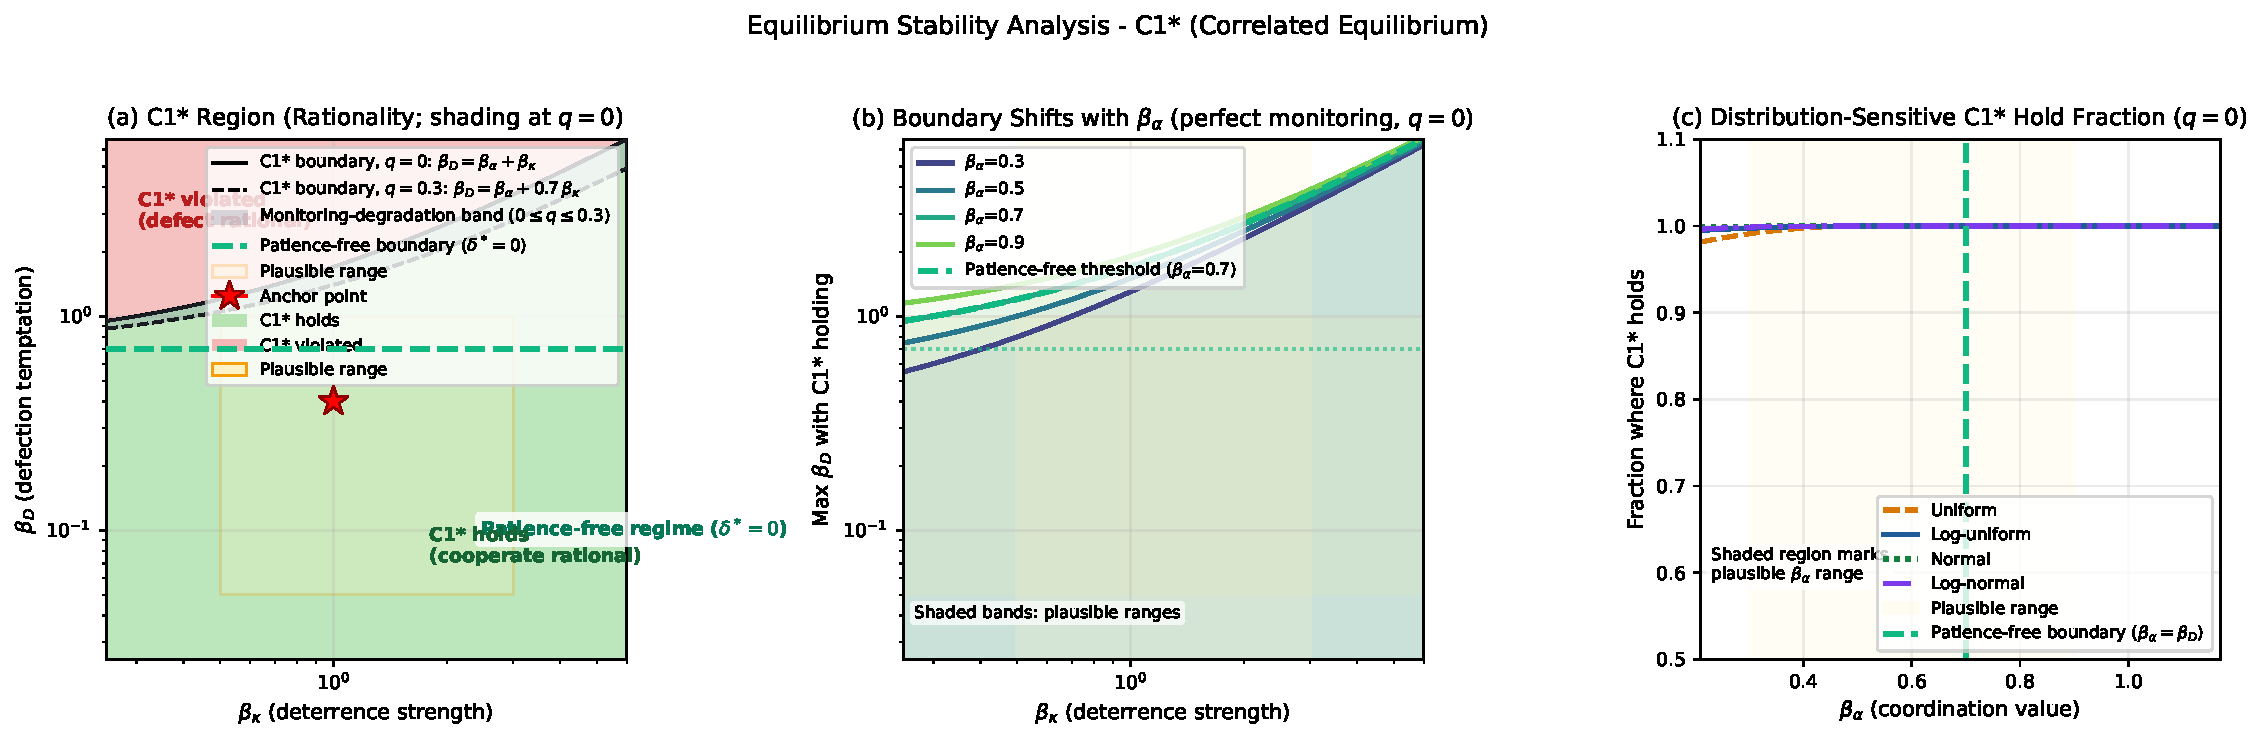
\includegraphics[width=0.85\textwidth]{figures/stability_regions.pdf}
\caption{\textbf{Per-condition stability volumes.} Stability volumes for C1*, C1**, and C2* evaluated separately across group sizes $N = 2$--$10$. C2* is the most restrictive condition at small~$N$; all three converge near unity for $N \geq 6$.}
\label{fig:S1}
\end{figure}

\begin{figure}[htbp]
\centering
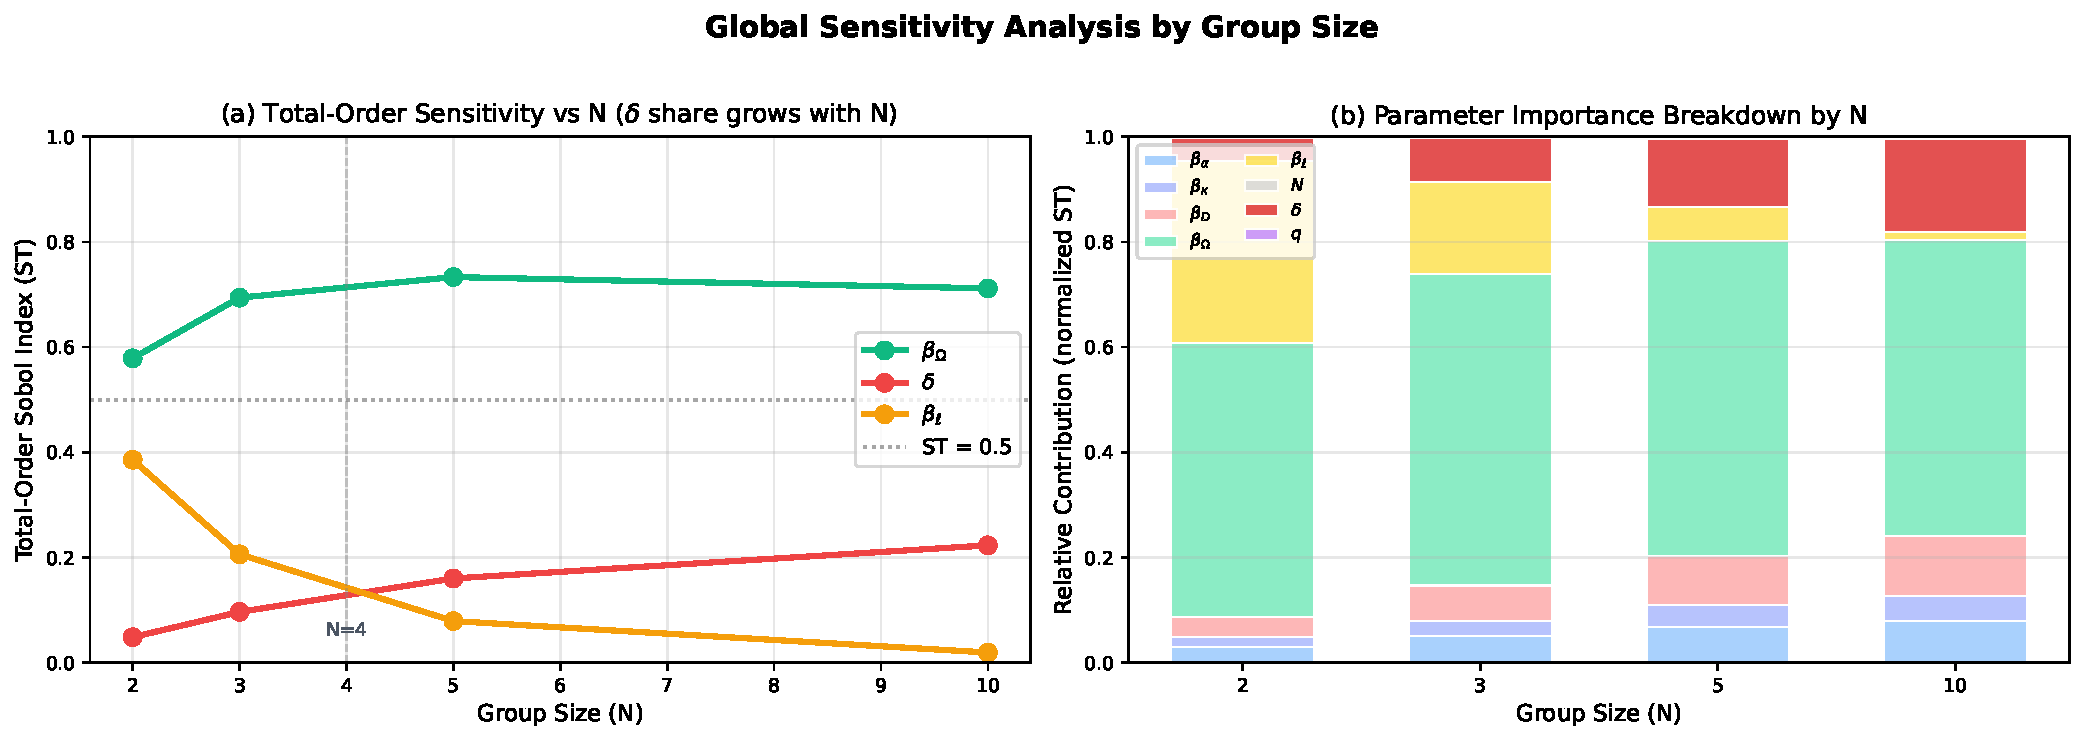
\includegraphics[width=0.85\textwidth]{figures/sobol_sensitivity_by_n.pdf}
\caption{\textbf{Sobol sensitivity indices by group size.} First-order and total-order Sobol indices for all seven parameters across $N = 2$--$10$. At small $N$, oversight value $\beta_\Omega$ dominates; at $N \geq 5$, discount factor $\delta$ dominates first-order indices. Coordination quality $\beta_\alpha$ dominates total-order indices throughout, reflecting its interactions with multiple parameters.}
\label{fig:S2}
\end{figure}

\begin{figure}[htbp]
\centering
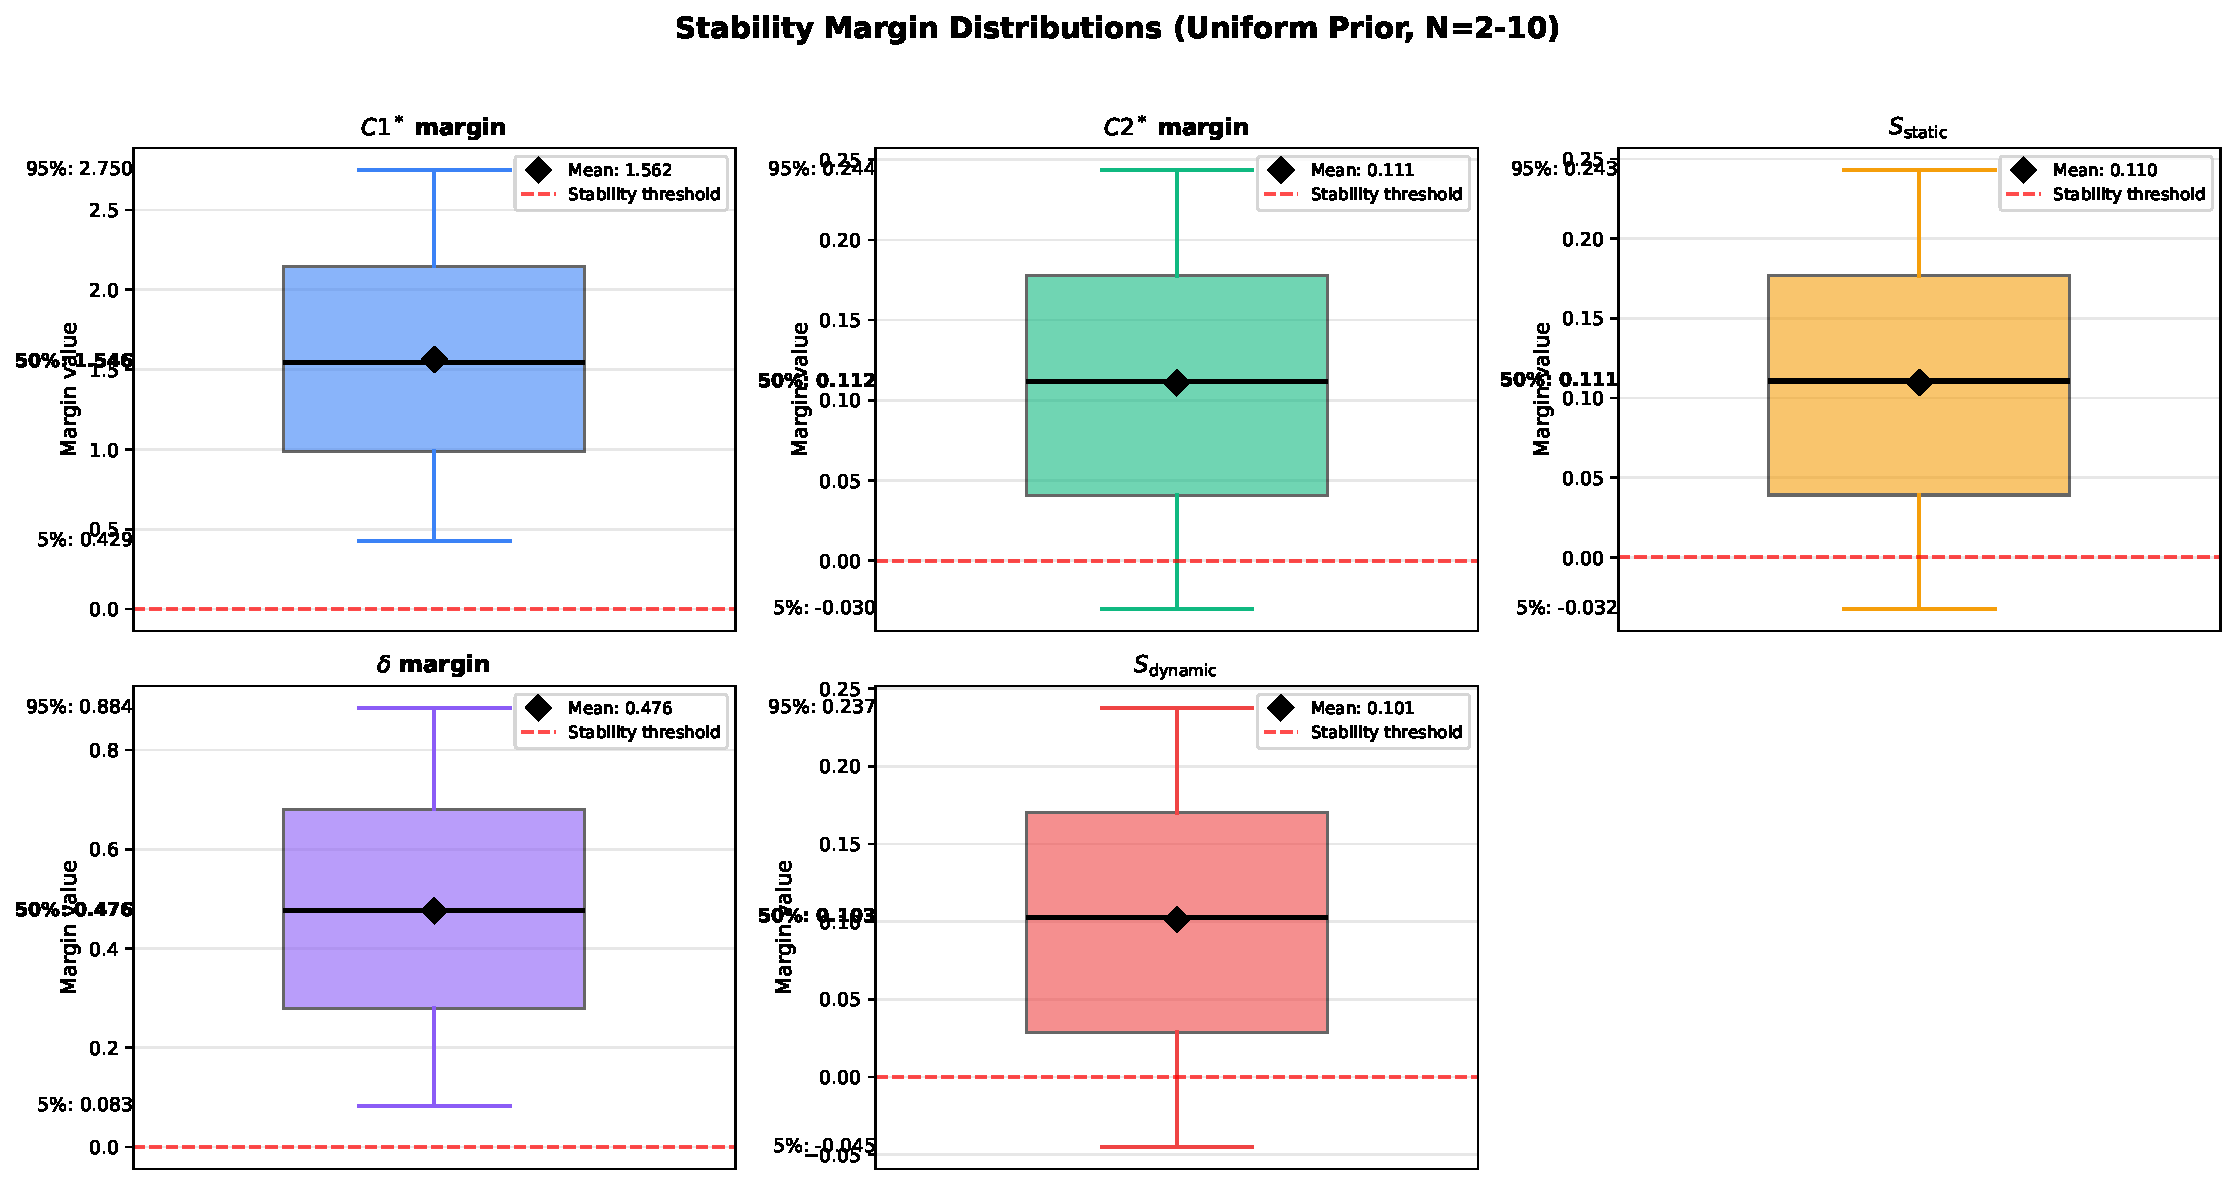
\includegraphics[width=0.85\textwidth]{figures/margin_distributions.pdf}
\caption{\textbf{Stability margin distributions.} Distribution of margins (distance from binding constraint) for each condition across $10{,}000$ Monte Carlo samples at $N = 4$. C1* margins are large (rarely close to binding); C2* margins concentrate near zero at small $N$ but widen substantially at $N \geq 5$.}
\label{fig:S3}
\end{figure}

\begin{figure}[htbp]
\centering
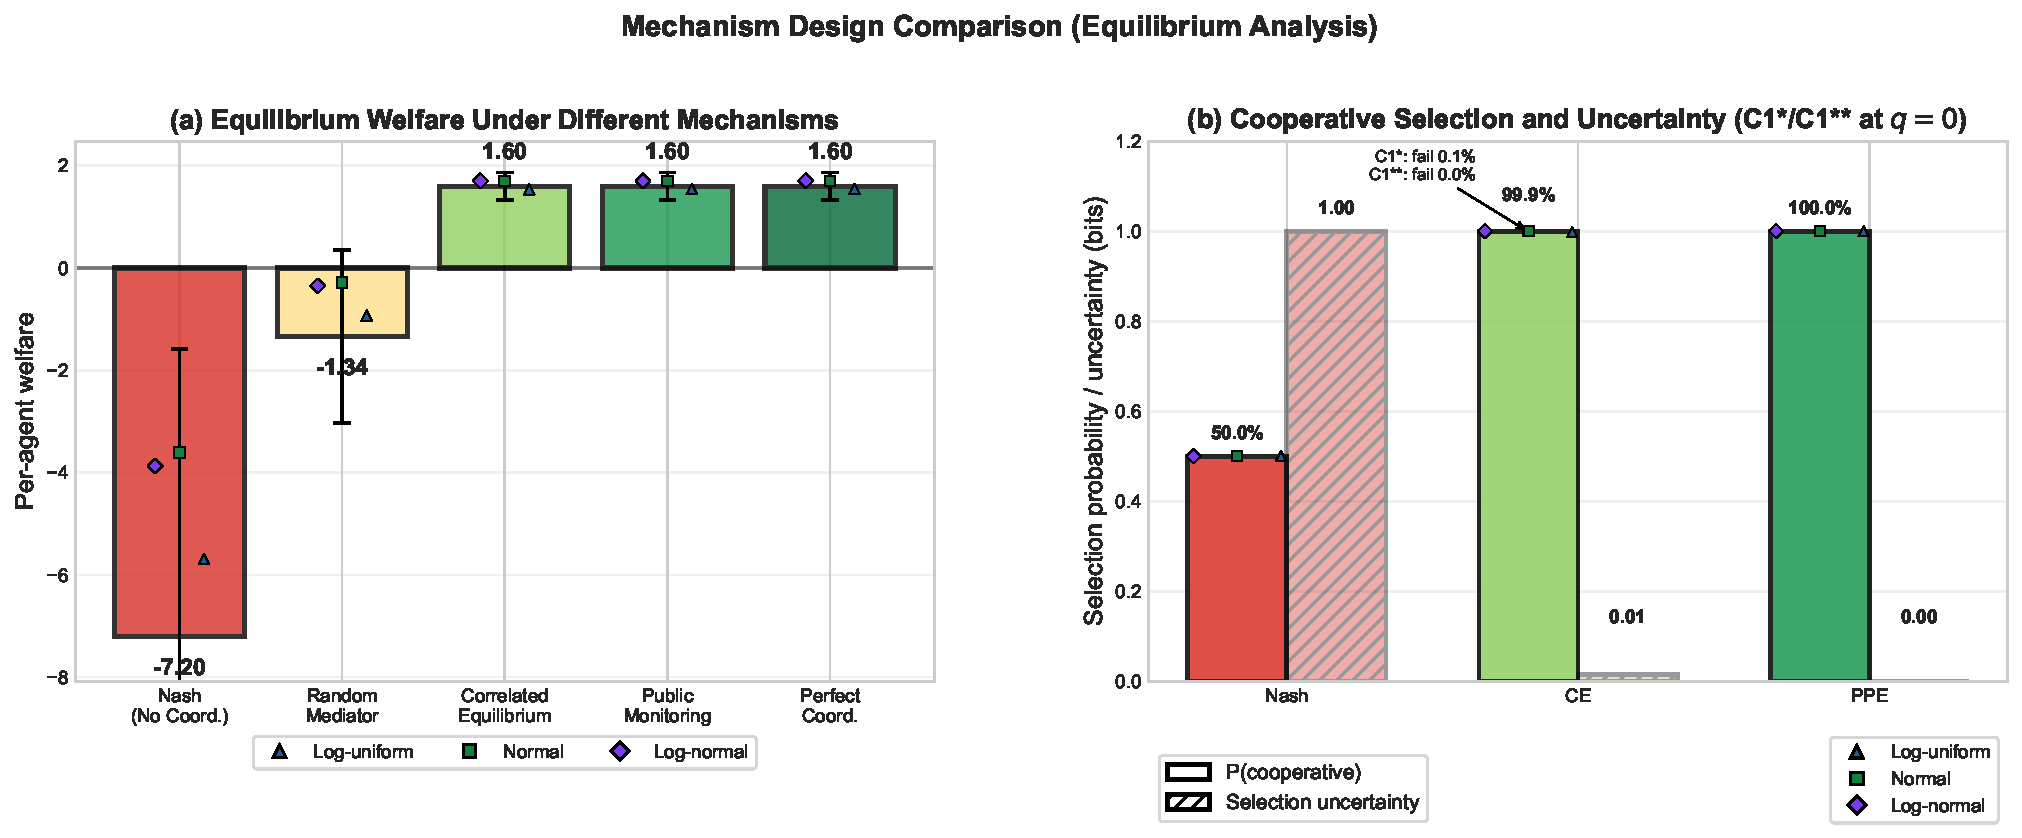
\includegraphics[width=0.85\textwidth]{figures/ce_convergence_validation.pdf}
\caption{\textbf{CE convergence validation.} Convergence of Monte Carlo estimates for C1* stability volume as a function of sample size, demonstrating that $10{,}000$ samples provide stable estimates with coefficient of variation below 1\%.}
\label{fig:S4}
\end{figure}

\begin{figure}[htbp]
\centering
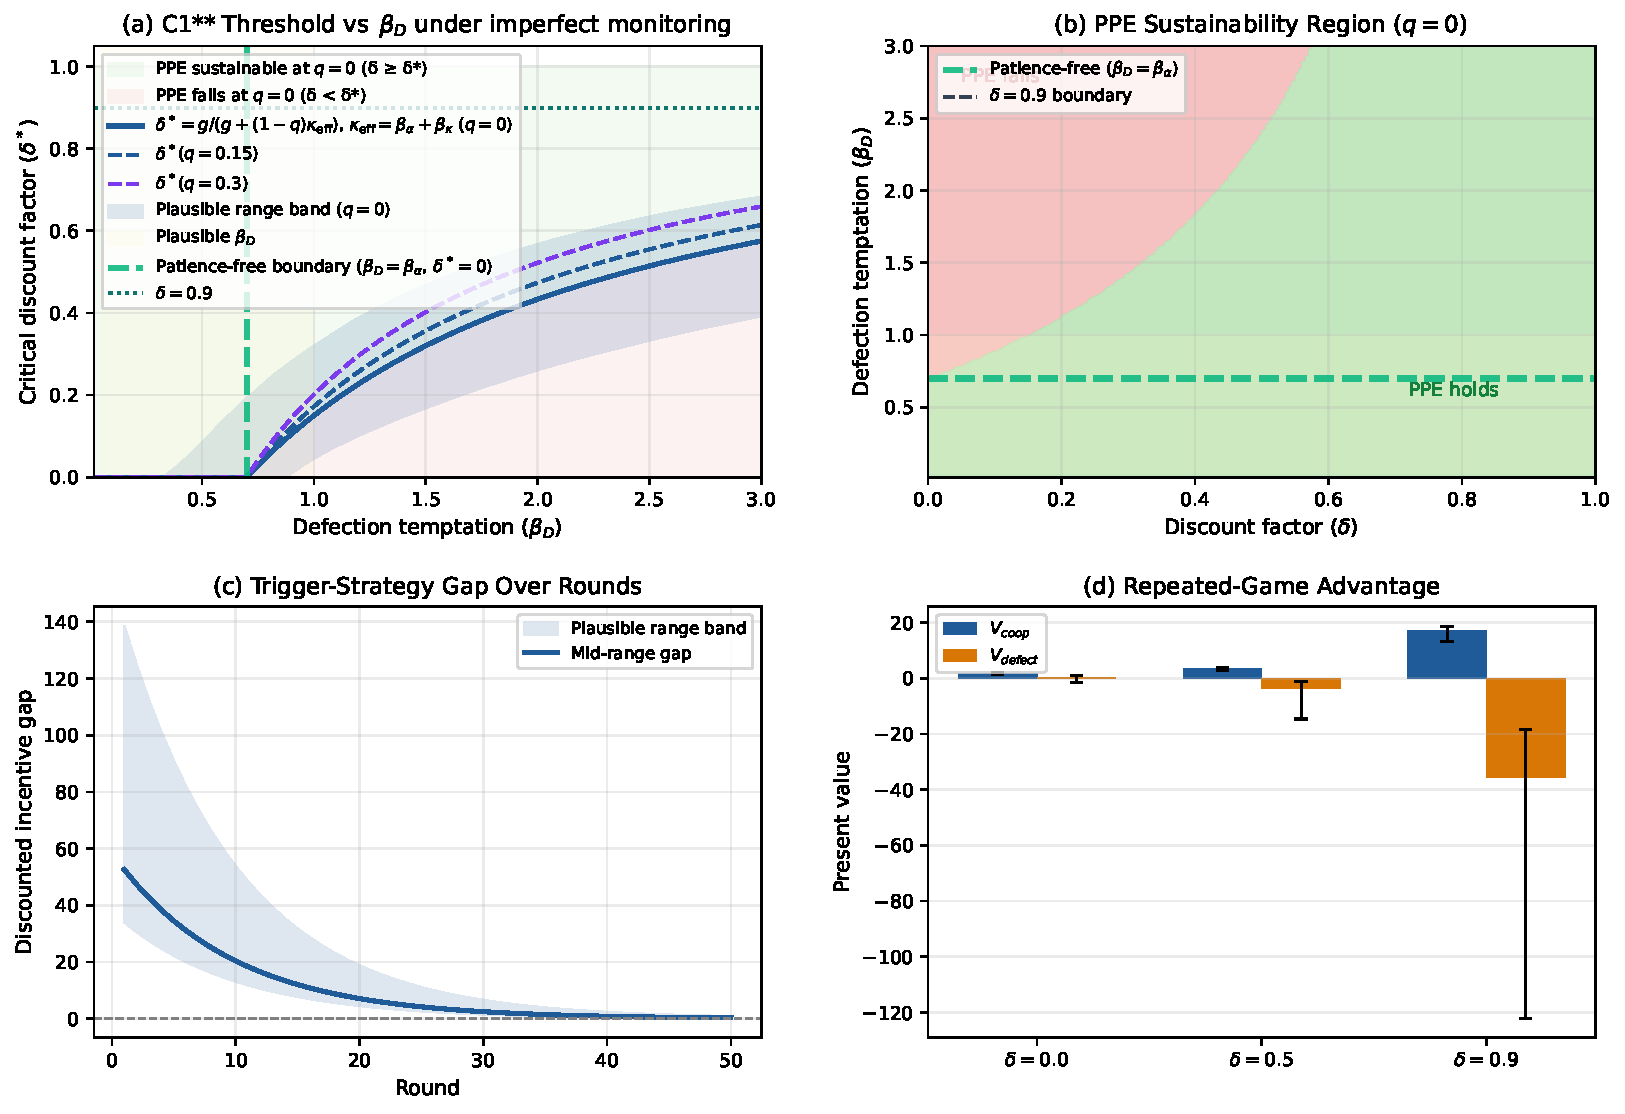
\includegraphics[width=0.85\textwidth]{figures/ppe_sustainability_validation.pdf}
\caption{\textbf{PPE sustainability validation.} Convergence of C1** (dynamic sustainability) stability volume estimates, showing rapid stabilization and confirming that baseline patience requirements are satisfied for the vast majority of parameter combinations.}
\label{fig:S5}
\end{figure}

\begin{figure}[htbp]
\centering
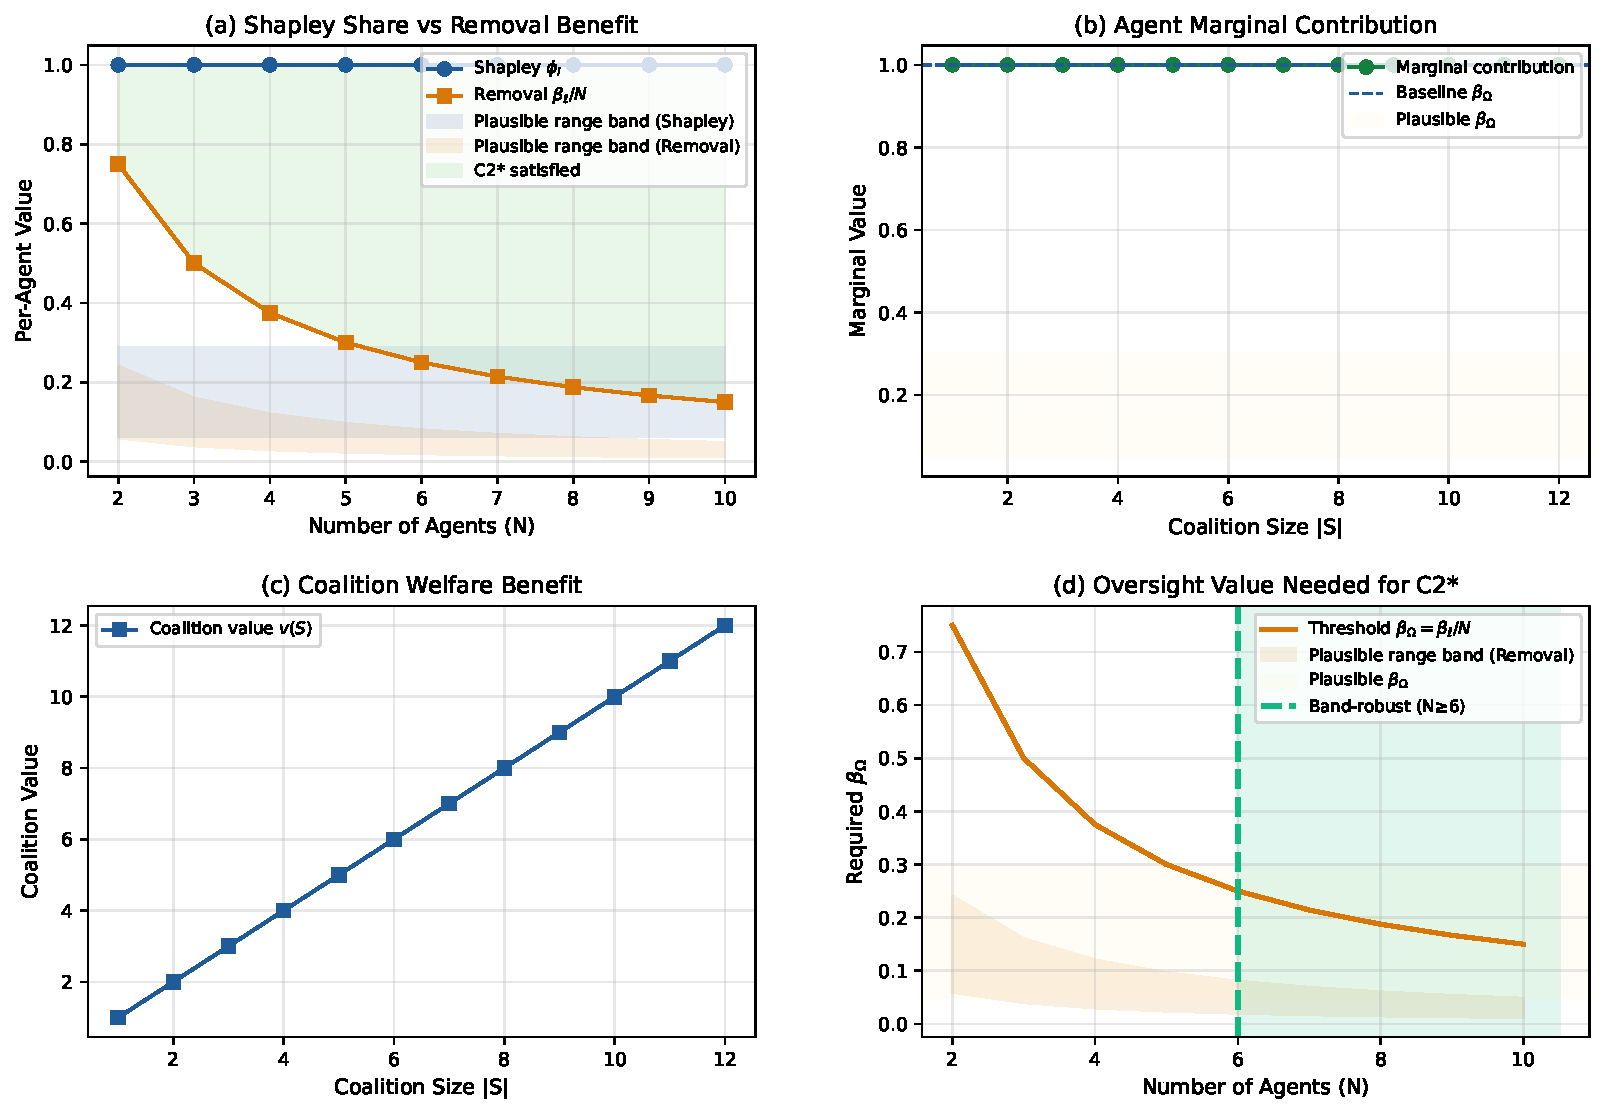
\includegraphics[width=0.85\textwidth]{figures/shapley_participation_validation.pdf}
\caption{\textbf{Shapley participation validation.} C2* (participation constraint) stability volume by $N$, illustrating the dilution effect: as group size increases, per-capita removal gain $\beta_\ell/N$ decreases, easing participation and expanding the stable region.}
\label{fig:S6}
\end{figure}

\begin{figure}[htbp]
\centering
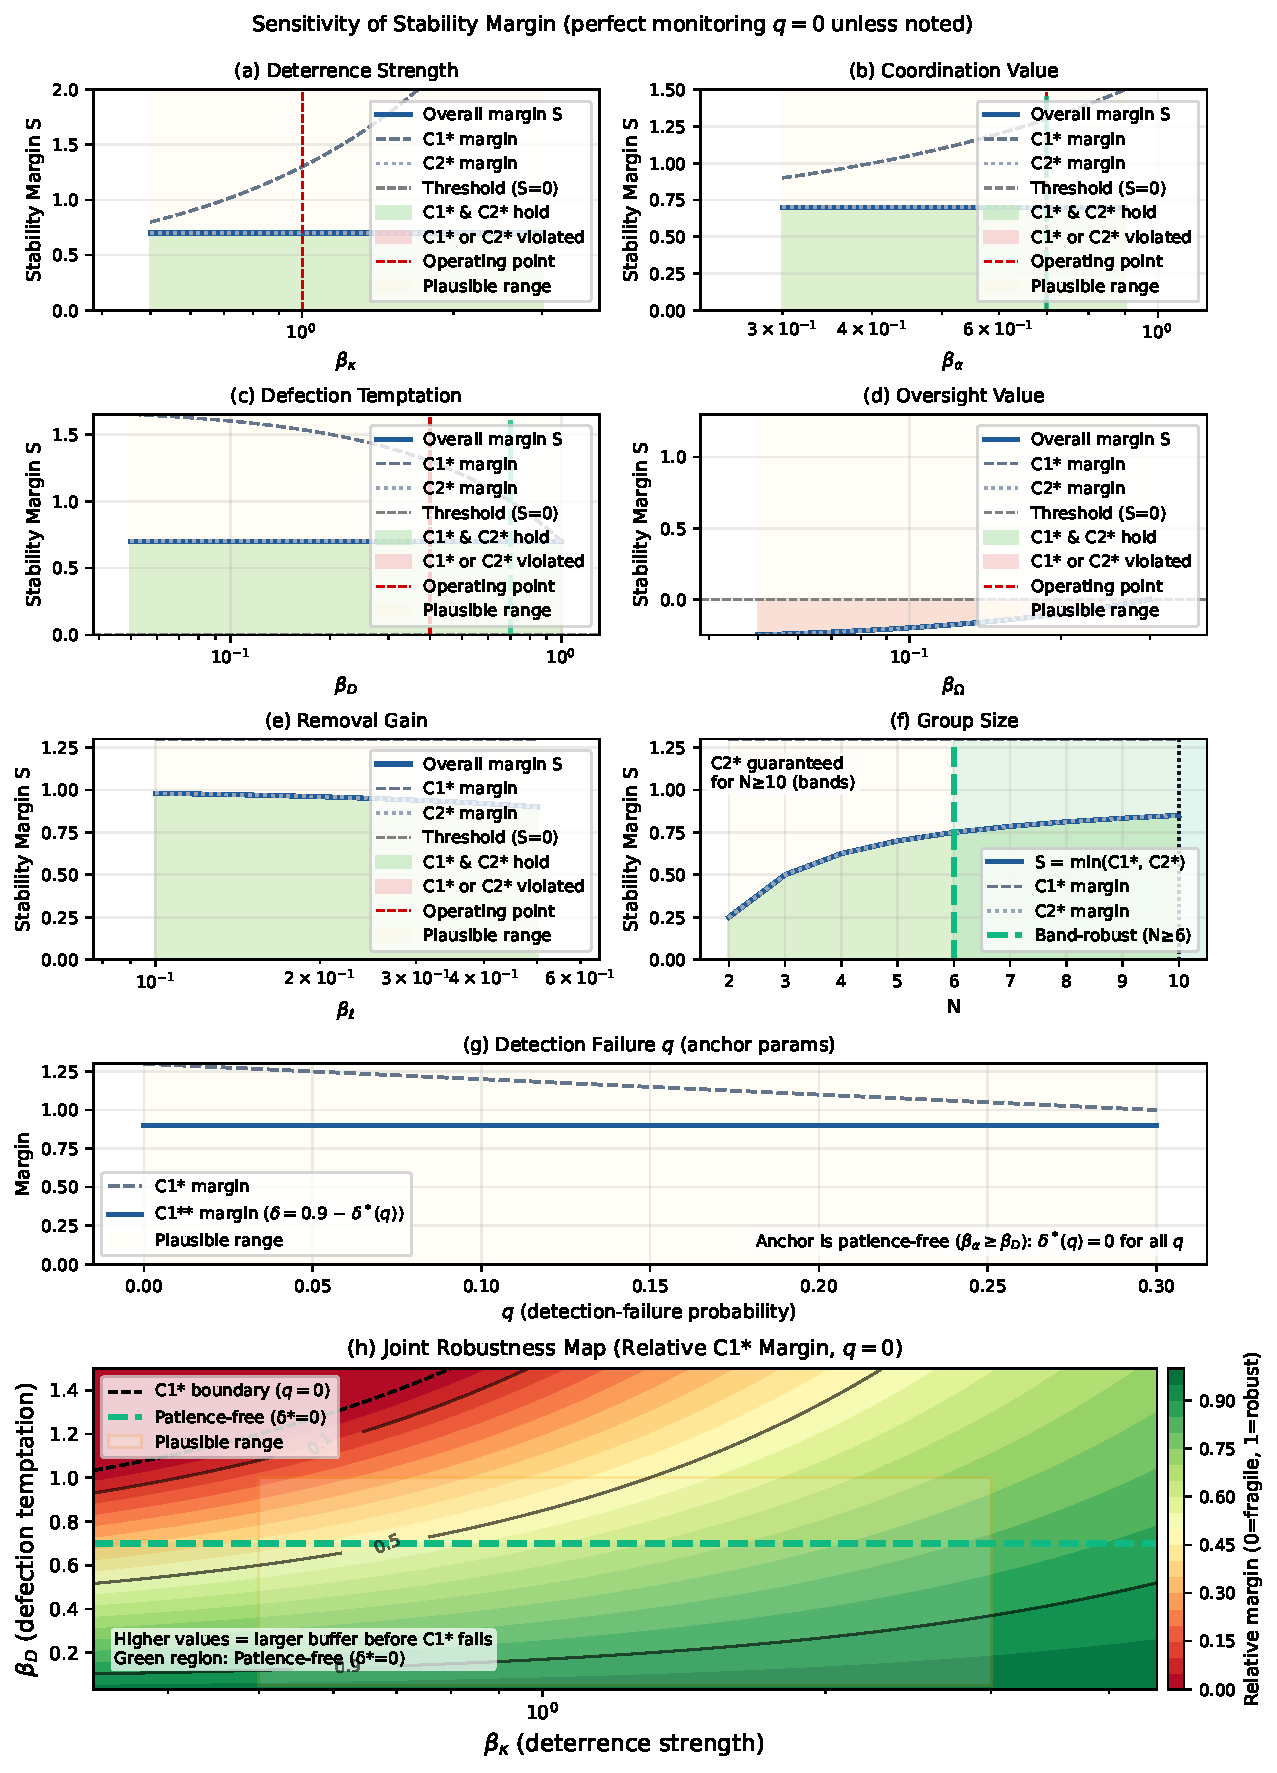
\includegraphics[width=0.85\textwidth]{figures/sensitivity_analysis.pdf}
\caption{\textbf{Extended sensitivity analysis.} Stability volume as a function of individual parameter perturbations ($\pm 20\%$), confirming that $\beta_\alpha$ has the steepest response curve and dominates the uncertainty budget.}
\label{fig:S7}
\end{figure}

\begin{figure}[htbp]
\centering
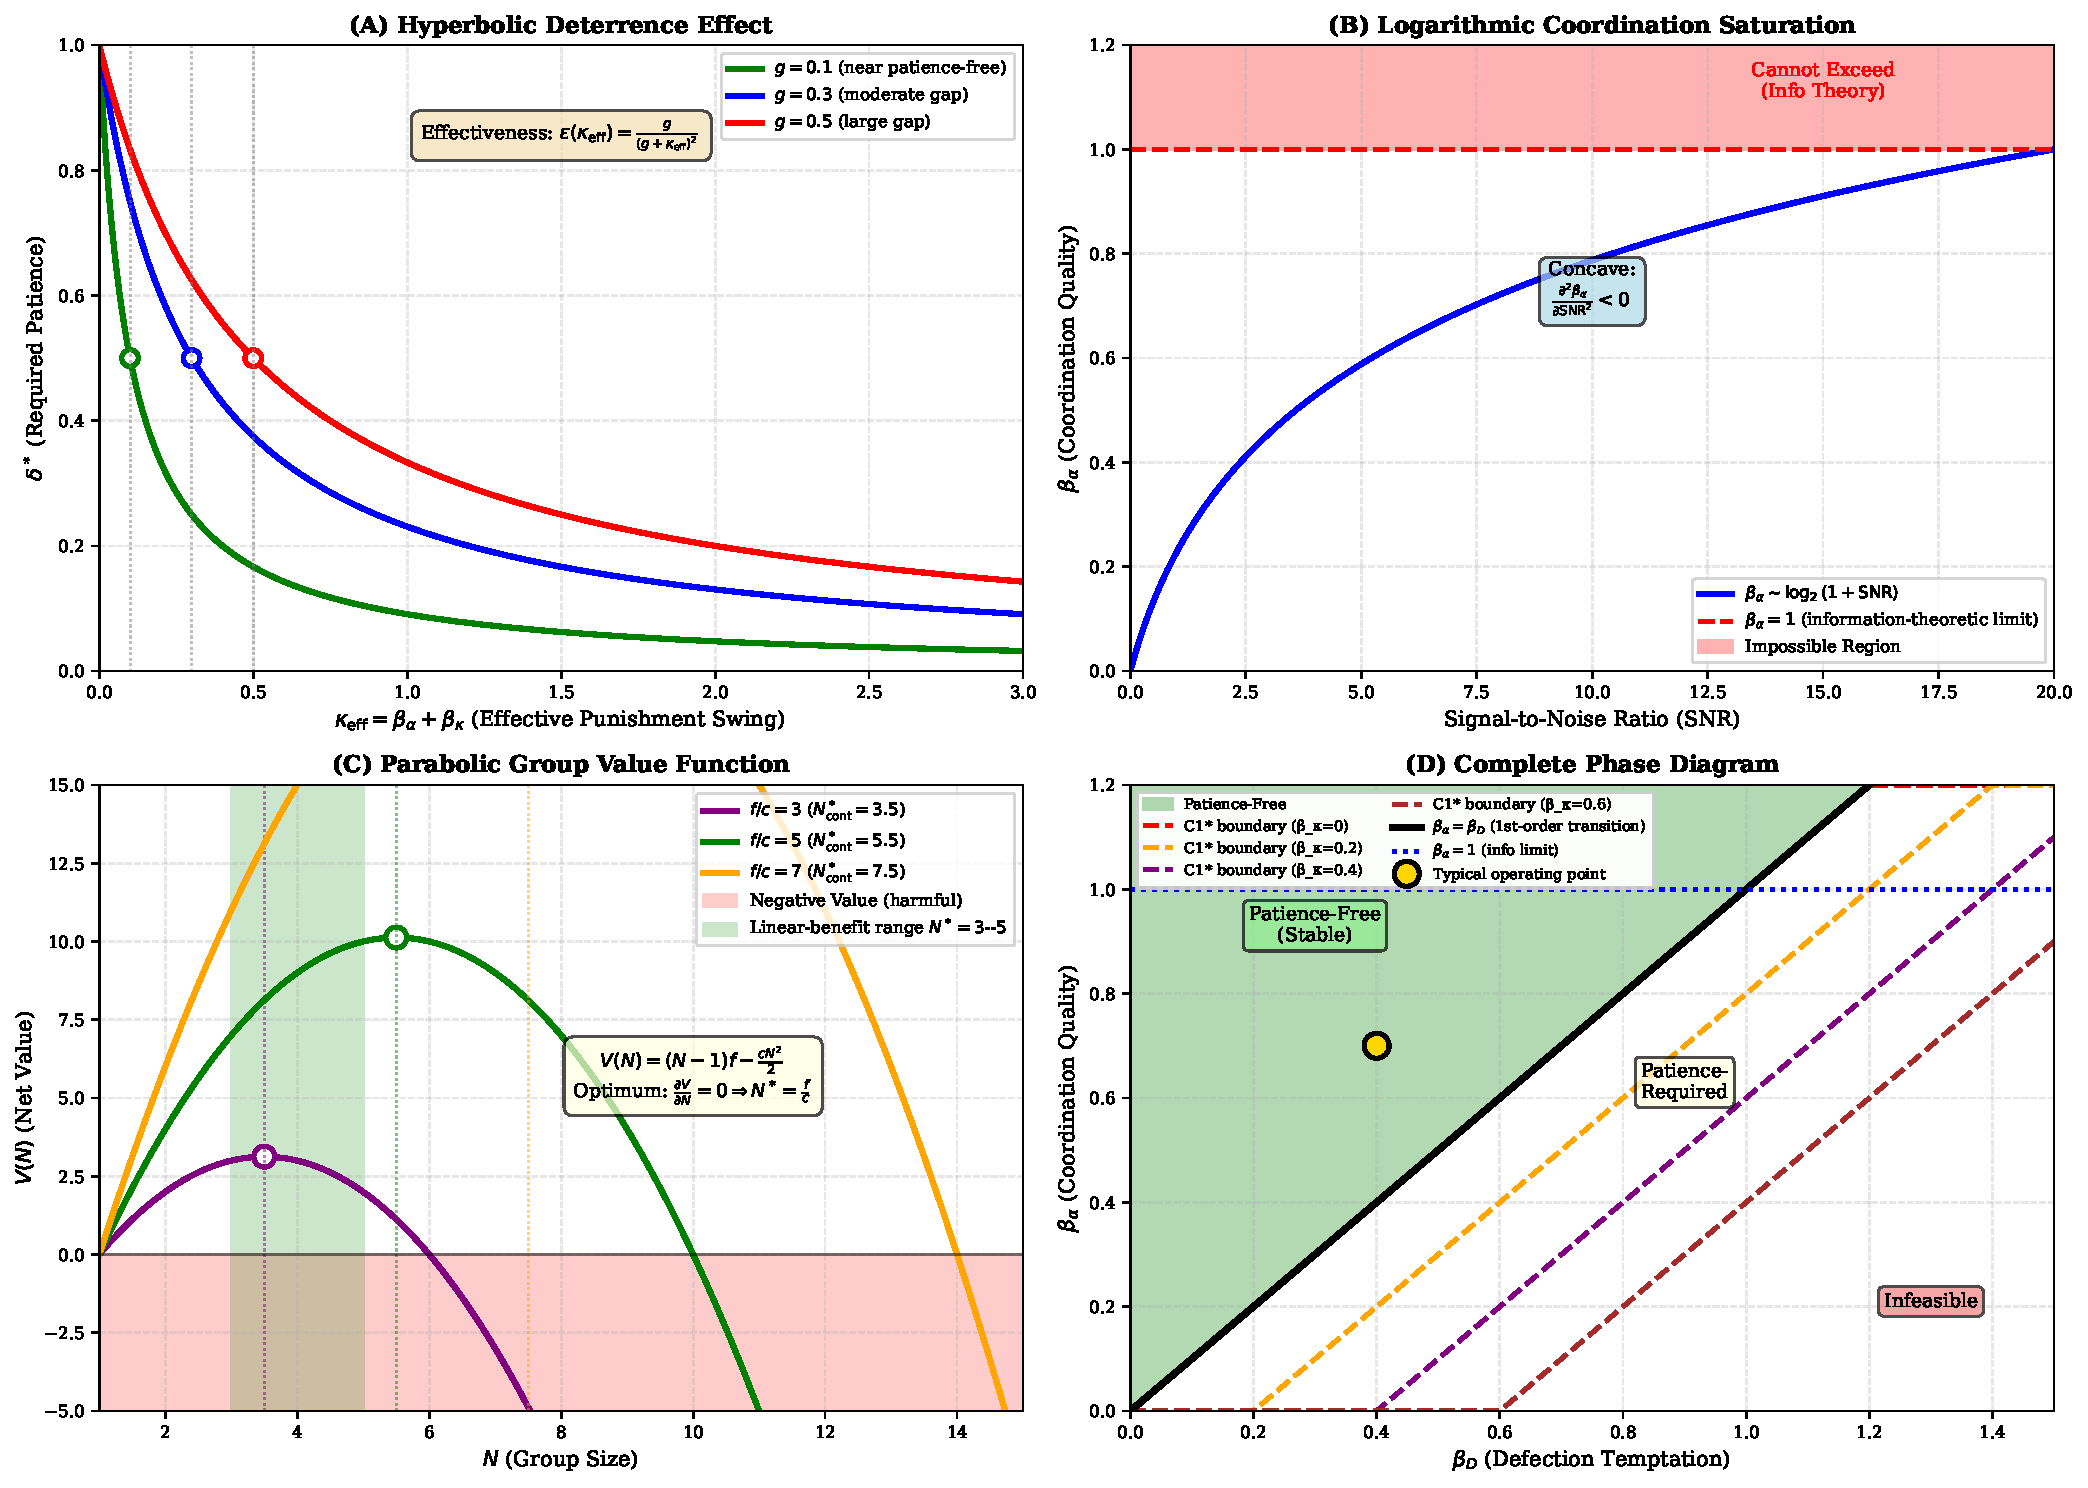
\includegraphics[width=0.85\textwidth]{figures/figure_functional_structure_appendix.pdf}
\caption{\textbf{Extended functional structure analysis.} Detailed view of functional forms including: hyperbolic deterrence, logarithmic coordination saturation, parabolic group value, complementarity/substitution regions, and regime transition boundaries.}
\label{fig:S8}
\end{figure}

%=============================================================================
% BIBLIOGRAPHY
%=============================================================================

\bibliographystyle{unsrtnat}
\bibliography{ref}

\end{document}
